\documentclass{beamer}
\usepackage{graphicx,url}
\usepackage{amsmath}
\usepackage{amssymb}
\usepackage{xkeyval}
\usepackage{multirow}
\usepackage{mytikz}
\usepgflibrary{shapes}
\usepackage{basics}
\usepackage{basics-slides}
\renewcommand{\emph}[1]{\alert{#1}}


%%%%%%%%%%%% Setting up MMTTeX

% path for background knowledge
\newcommand{\mmttexmathhubroot}{c:/other/oaff/}
% import the package
\usepackage{../latex/mmttex}

% add lexing rules for Unicode (talk about it later)
\mmtUnicodeAsAscii
\mmtUnicodeAsLatex

% define a namespace abbreviation for modules in the background knowledge
\mmtimport{ex}{http://cds.omdoc.org/examples}

\begin{document}

\title{System Description: MMTTeX \\ \small Connecting Content and Narration-Oriented Document Formats}
\author{Florian Rabe}
\institute{Computer Science, University Erlangen-N\"urnberg, Germany \\ LRI, University Paris-Sud, France}
\date{July 2019}
\begin{frame}
    \titlepage
\end{frame}


%%%%%%%%%%%%%%%%%%%%%%%%%%%%%%%%%%%%%%%%%%%%
\section{Motivation}

\begin{frame}\frametitle{Subsume All Aspects of Knowledge}
\begin{itemize}
\item Narration: informal-but-rigorous math
  \lec{needed for human consumption}
\item Deduction: logic and type systems
  \lec{needed for machine understanding}
\item Computation: data structures and algorithms
  \lec{needed for practical applications}
\item Data: tabulate large sets and functions
  \lec{needed for examples, exploration and efficiency}
\item<2> Universal representation language
 \lec{key to universality, inter-operability}
\end{itemize}

\begin{center}
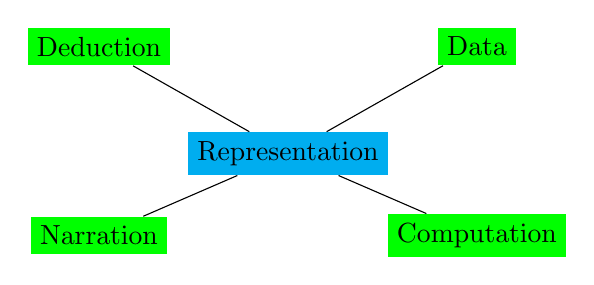
\begin{tikzpicture}[scale=.8]
\node[fill=green] (D)  at (-3,3)   {Deduction};
\node[fill=green] (T)  at (3,3)    {Data};
\node[fill=green] (Cm)  at (3,0)   {Computation};
\node[fill=green] (N)  at (-3,0)   {Narration};

\node[fill=cyan] (Cn)  at (0,1.3)   {Representation};
\draw[-] (Cn) -- (D);
\draw[-] (Cn) -- (T);
\draw[-] (Cn) -- (Cm);
\draw[-] (Cn) -- (N);
\end{tikzpicture}
\end{center}
\end{frame}

\begin{frame}\frametitle{MMT as System Integration Platform}
All system interfaces formalized in MMT \\
$\to$ semantics-aware tool integration while maintaining existing work flows
\begin{center}
\begin{tikzpicture}[xscale=1.5]
\tikzstyle{conn}=[angle 45-angle 45]
\tikzstyle{field}=[draw,rectangle]

\node[field] (KM) at (0,2.8)  {Data, tables};
\node[field] (Spec) at (0,-2.8)  {Narration, documents};
\node[field,rotate=-90] (Spec) at (3.7,0)  {Computation, programs};
\node[field,rotate=90] (Ded) at (-3.3,0)  {Deduction, proofs};

\node[draw,ellipse] (U) at (0,0)  {MMT as Mediator};
\node (Sp) at (1,-2)  {WWW};
\node (TP) at (-2,-1)  {Specification};
\node (PA1) at (-2,.7)  {Provers};
\node (PA2) at (-2,1.3)  {Model checkers};
\node (CAS) at (2.5,.5)  {Symbolic comp.};
\node (Op) at (2,1.3)  {Numeric comp.};
\node (Sa) at (2,-.7)  {Progr. lang.};
\node (Sc) at (2,-1.3)  {Program synthesis};
\node (M) at (-1,2)  {Math databases};
\node (MWS) at (1,2)  {Query Languages};

\only<2>{\begin{scope}[red]}
\node (He) at (-1,-2)  {\LaTeX};
\draw[conn](U) -- (He);
\node (tt) at (-2,-2) {this talk};
\only<2>{\end{scope}}

\draw[conn](U) -- (Sp);
\draw[conn](U) -- (M);
\draw[conn](U) -- (MWS);
\draw[conn](U) -- (Op);
\draw[conn](U) -- (CAS);
\draw[conn](U) -- (Sa);
\draw[conn](U) -- (Sc);
\draw[conn](U) -- (TP);
\draw[conn](U) -- (PA1);
\draw[conn](U) -- (PA2);
\end{tikzpicture}
\end{center}
\end{frame}

\section{Design}

\begin{frame}\frametitle{Ideal System}
Requirements:
\begin{itemize}
\item Author flexibly switches between MMT and LaTeX
 \begin{itemize}
 \item multiple nesting levels allowed
 \item top level can be either format
 \end{itemize}
\item Control passes between MMT and LaTeX processor
 \begin{itemize}
 \item sharing the same context
 \item communicating context changes
 \end{itemize}
  \glec{e.g., introduce name in MMT chunk, use it in LaTeX chunk}
\item Produces OMDoc, pdf, HTML, etc.
\end{itemize}

Problems:
\begin{itemize}
\item No way to get LaTeX processor to interact flexibly
\item No way to write a new LaTeX processor for the occasion
\end{itemize}
\end{frame}

\begin{frame}\frametitle{Realistic Options}
\begin{blockitems}{Symmetric}
\item new document format with new processor
\item interspersed MMT and LaTeX chunks
\item generate \texttt{.tex} and \texttt{.mmt} files, process separately, merge the outputs into OMDoc
\end{blockitems}
\lec{failed 2016 CICM submission}

\begin{blockitems}{MMT-led}
\item .mmt file processed by MMT
\item interspersed LaTeX chunks
\item MMT generates \texttt{.tex} file
\end{blockitems}

\begin{blockitems}{LaTeX-led}
\item .tex file processed by LaTeX
\item interspersed MMT chunks
\item LaTeX generates \texttt{.mmt} file
\end{blockitems}
\lec{\color{red}this talk}
\end{frame}

\begin{frame}\frametitle{Work flow}
2 components using BibTeX model

\begin{itemize}
\item \texttt{mmttex.sty} package for LaTeX
 \begin{itemize}
 \item first run: writes out MMT chunks to \texttt{d.tex.mmt}
 \item second run: replaces MMT chunks with code from \texttt{d.tex.sty}
 \end{itemize}
\item \texttt{latex-mmt} plugin for MMT
 \begin{itemize}
 \item processes \texttt{d.tex.mmt} as usual
 \item generates \texttt{d.tex.sty} with special LaTeX code
 \end{itemize}
\end{itemize}

\begin{center}
\begin{tabular}{|l||l|l|l|}
\hline
& Input & Processor & Output \\
\hline
\hline
Step 1 & \texttt{d.tex} & LaTeX & \texttt{d.pdf} \\
       &                &       & \texttt{d.tex.mmt}\\
\hline
Step 2 & \texttt{d.tex.mmt} & MMT & \texttt{d.tex.omdoc} \\
       &                    &     & \texttt{d.tex.sty}\\
\hline
Step 3 & \multicolumn{3}{c|}{Run LaTeX again} \\
\hline
\end{tabular}
\end{center}
\end{frame}

\begin{frame}\frametitle{Advantages}
Semantics-aware formula processing
\begin{itemize}
\item MMT parsing and type-checking
\item semantic errors in MMT content produce LaTeX compilation errors
\item formulas enriched with inferred information
 \lec{implicit arguments, omitted types}
\end{itemize}

Semantically enriched formulas in \texttt{.pdf}
\begin{itemize}
\item tooltips on symbols
\item hyper-references from usage to definition
\item whatever else we can get the pdf viewers to support
 \lec{e.g., JavaScript barely supported}
\end{itemize}
\end{frame}


\begin{frame}\frametitle{3 kinds of MMT content}
\begin{center}
\begin{tabular}{|l||l|l|l|}
\hline
Kind & defined in & function \\
\hline
\hline
Pres.-rel. chunks   & \multirow{2}{*}{LaTeX document}  & payload\\
\cline{1-1}\cline{3-3}
Pres.-irrel. chunks &  & \multirow{2}{*}{needed by payload}\\
\cline{1-2}
Backgr. Knowledge         & elsewhere & \\
\hline
\end{tabular}
\end{center}

\begin{itemize}
\item Presentation-\textbf{relevant} MMT chunks
 \begin{itemize}
 \item formulas defined in MMT instead of LaTeX syntax
 \item produce semantically enriched formulas in the \texttt{.pdf} file
 \end{itemize}
 \lec{e.g., $2+2=4$}
\item Presentation-\textbf{irrelevant} MMT chunks
 \begin{itemize}
 \item provide context for the pres.-rel. chunks
 \item part of \texttt{.tex} file
 \item no effect on \texttt{.pdf} file
 \end{itemize}
  \lec{e.g., definition of $+$}
\item Background knowledge
 \begin{itemize}
 \item available in MMT independent of LaTeX document
 \item define formal language(s) used in \texttt{tex} file
 \end{itemize}
 \lec{e.g., formalization of logic, including $=$}
\end{itemize}
\end{frame}

\section{Example and Demo}

\begin{frame}\frametitle{Game Plan}
\begin{itemize}
\item Background knowledge: typed first-order logic in MMT
\item Write a LaTeX document using MMTTeX
 \lec{these slides themselves!}
 \begin{enumerate}
  \item define theory of groups
  \begin{itemize}
   \item informally as usual
   \item additional pres.-irrel. chunks for formalization
  \end{itemize}
  \item write formulas about groups in formal MMT syntax
 \end{enumerate}
\end{itemize}
\end{frame}


%%%%%%%%%%%%%%%%%%%%%%%%%%%%%%%%%%%%%%%%%%%%


\begin{frame}\frametitle{Groups}

\begin{mmttheory}{Group}{ex:?SFOLEQ}

A group consists of
\begin{itemize}
\item a set $U$,
\mmtconstant{U}{tp}{}{}

\item an operation $U\to U \to U$, written as infix $*$,
\mmtconstant{operation}                % name
            {tm U --> tm U --> tm U}   % type
            {}                         % definiens
            {1 * 2 prec 50}            % notation

\item an element $e$ of $U$ called the unit
\mmtconstant{unit}{tm U}{}{e}

\item an inverse element function $U\to U$, written as postfix $'$ and with higher precedence than $*$.
\mmtconstant{inv}{tm U --> tm U}{}{1 ' prec 60}
\end{itemize}
We omit the axioms.
\bigskip

\begin{mmtcontext}
Consider group elements \mmtvar{a}{tm U} and \mmtvar{b}{tm U}.

Then we define the division of "a" by "b" as "a*b'".
\end{mmtcontext}

\end{mmttheory}

\end{frame}


\begin{frame}\frametitle{Division}

We extend the theory of groups with a defined operation for division written as a fraction.
\begin{mmttheory}{Division}{ex:?SFOLEQ}
\mmtinclude{?Group}
\mmtconstant{division}{tm U --> tm U --> tm U}{[x,y] x*y'}{1 / 2 prec 50}
\bigskip

Now we can prove "\forall [x] x / x =. e".
\end{mmttheory}
\end{frame}


%%%%%%%%%%%%%%%%%%%%%%%%%%%%%%%%%%%%%%%%%%%%
\section{Conclusion}


\begin{frame}[fragile]\frametitle{Sidenote: Call for Help}
How do I make LaTeX forward a Unicode symbol unchanged to the generated \texttt{.mmt}?
\bigskip

I have a macro \verb|\toMMT{#1}| that
\begin{itemize}
 \item appends \verb|#1| to the \texttt{.mmt} file
 \item does not produce any output for the \texttt{.pdf} file
\end{itemize}

But it goes haywire if \verb|#1| contains Unicode characters.
\bigskip

Current workaround:
\begin{itemize}
\item avoid Unicode in MMT chunks
\item if required by background knowledge, add parsing rules\\
 e.g., MMT can parse \verb|->| or \verb|\rightarrow| as $\rightarrow$
\end{itemize}
\end{frame}

\begin{frame}\frametitle{Prior Attempts}
Two predecessors (papers rejected, systems abandoned)
\begin{blockitems}{CICM 2013: with M. Iancu, D. Ginev}
  \item also LaTeX-led but with single LaTeX run only
  \item LaTeX talked to MMT dynamically via HTTP
  \item main problem: badly chosen story, LaTeX run with \texttt{shell-escape} flag
\end{blockitems}

\begin{blockitems}{CICM 2016: with M. Iancu, M. Kohlhase, H. Yuan}
  \item symmetric design
  \item general infrastructure
  \item arbitrary nesting of MMT and LaTeX
  \item MMT and LaTeXML output merged into OMDoc
  \item main problem: complex design hard to implement
\end{blockitems}
Current paper: much narrower focus, much simpler system
\end{frame}

\begin{frame}\frametitle{Summary}
\begin{itemize}
 \item First step towards integration of LaTeX and MMT
  \lec{type-checking while type-setting}
 \item Semantic analysis and enriched presentation of formulas
 \item Very simple system
 \item Easy to extend by users
  \begin{itemize}
  \item new background knowledge using logical frameworks in MMT
  \item new LaTeX macros for writing and displaying MMT content
  \item variants of MMT plugin for more semantic enrichment
  \end{itemize}
 \item Future work
  \begin{itemize}
  \item use MitM as default background knowledge library
  \item use MMT also for definitions, proofs, \ldots
  \item combine with MMT-led integration
  \end{itemize}
\end{itemize}
\end{frame}
%%%%%%%%%%%%%%%%%%%%%%%%%%%%%%%%%%%%%%%%%%%%

\end{document}

